\documentclass[pra,aps,10pt,twocolumn,floatfix,superscriptaddress,
notitlepage,longbibliography]{revtex4-2}

\usepackage{xcolor, soul}

% -------------------------------------------------------
% PACKAGES
% -------------------------------------------------------
\usepackage[T1]{fontenc}
\usepackage[utf8]{inputenc}
\usepackage{graphicx,color}
\usepackage{amsmath,amssymb,amsfonts}
\usepackage{quantikz}
\usepackage{amsthm}
\usepackage{subcaption}
\newtheorem{definition}{Definition}
\usepackage{bm}
\usepackage[linesnumbered,ruled,vlined]{algorithm2e}
\usepackage[noend]{algpseudocode}
\usepackage[colorlinks=true,citecolor=blue,linkcolor=magenta,urlcolor=blue]{hyperref}
\usepackage{braket}
\usepackage{tikz}
\usepackage{booktabs}
\usepackage{multirow}
\usepackage{siunitx}
\usepackage{eurosym}

\sisetup{
  detect-mode,
  table-format=1.4,
  table-number-alignment = center
}

\newtheorem{proposition}{Proposition}
\newtheorem{theorem}{Theorem}
\newtheorem{lemma}{Lemma}
\newtheorem{corollary}{Corollary}
\newcommand{\bits}{\{0,1\}}
\newcommand{\E}{\mathbb{E}}
\newcommand{\mmd}{\operatorname{MMD}}
\newcommand{\TVD}{\operatorname{TVD}}
\newcommand{\supp}{\operatorname{supp}}
\makeatletter
\newcommand{\tableinput}[1]{\@@input #1 }
\makeatother
\definecolor{paperblue}{HTML}{0072B2}
\newenvironment{plainwidetext}{\par\onecolumngrid\vspace{4pt}}{%
  \par\vspace{4pt}\twocolumngrid}
\newcommand{\widefigurecaption}[2]{%
  \refstepcounter{figure}\label{#2}%
  \par\vspace{6pt}
  \noindent\parbox{\textwidth}{\small Figure~\thefigure: #1}\par}

\newif\ifgaussianresults
\IfFileExists{generated/gaussian_claims.tex}{
  \gaussianresultstrue
  % Generated by scripts/finalize_gaussian_claims.py. Do not edit.
\newcommand{\GaussianAtomicModels}{1,020}
\newcommand{\GaussianManifestDigest}{386ce98be93501f078d45b29e7fa498db1600c44d0e22f4483c3c8d5c7ec0d8c}
\newcommand{\ProfileControlSupported}{12}
\newcommand{\ProfileControlMixed}{0}
\newcommand{\ProfileControlUnsupported}{0}
\newcommand{\ProfileLookupSupported}{0}
\newcommand{\ProfileLookupMixed}{2}
\newcommand{\ProfileLookupUnsupported}{10}
\newcommand{\ProfileMixtureSupported}{2}
\newcommand{\ProfileMixtureMixed}{1}
\newcommand{\ProfileMixtureUnsupported}{9}
\newcommand{\BitstringControlSupported}{12}
\newcommand{\BitstringControlMixed}{0}
\newcommand{\BitstringControlUnsupported}{0}
\newcommand{\BitstringLookupSupported}{2}
\newcommand{\BitstringLookupMixed}{1}
\newcommand{\BitstringLookupUnsupported}{9}
\newcommand{\HeadlineProfileControl}{0.2668 [0.2587, 0.2737]}
\newcommand{\HeadlineProfileBankGap}{0.0878 [0.0860, 0.0897]}
\newcommand{\HeadlineProfileLookup}{0.0016 [-0.0012, 0.0043]}
\newcommand{\HeadlineProfileMixture}{-0.0029 [-0.0053, -0.0006]}
\newcommand{\HeadlineBitstringLookup}{-0.0606 [-0.0749, -0.0461]}

}{
  \gaussianresultsfalse
  \newcommand{\GaussianAtomicModels}{0}
  \newcommand{\HeadlineProfileControl}{pending}
  \newcommand{\HeadlineProfileBankGap}{pending}
  \newcommand{\HeadlineProfileLookup}{pending}
  \newcommand{\HeadlineProfileMixture}{pending}
}

\IfFileExists{generated/curie_weiss_ancilla_claims.tex}{
  % Generated from all 80 immutable fixed-m=5 Curie--Weiss fits.
\newif\ifcurieweissancillaresults
\curieweissancillaresultstrue
\newcommand{\CWAncillaReportSHA}{ea95a0f33bacb43442077eb6c145123eb7125e32879e7c96d0893131f63c7465}
\newcommand{\CWAncillaAtomicFits}{80}
\newcommand{\CWAncillaProfileControlTraining}{+0.134 [+0.129, +0.140]}
\newcommand{\CWAncillaProfileControlHeldOut}{+0.121 [+0.116, +0.127]}
\newcommand{\CWAncillaRawControlTraining}{+0.140 [+0.135, +0.145]}
\newcommand{\CWAncillaRawControlHeldOut}{+0.128 [+0.123, +0.134]}
\newcommand{\CWAncillaProfileMixtureHeldOut}{-0.011 [-0.017, -0.005]}
\newcommand{\CWAncillaRawMixtureHeldOut}{+0.008 [+0.002, +0.013]}
\newcommand{\CWAncillaProfileOracleHeldOut}{+0.015 [+0.011, +0.019]}
\newcommand{\CWAncillaRawOracleHeldOut}{+0.036 [+0.031, +0.041]}
\newcommand{\CWAncillaProfileCritical}{+0.038 [+0.030, +0.047]}
\newcommand{\CWAncillaRawCritical}{+0.056 [+0.048, +0.065]}
\newcommand{\CWAncillaProfileCold}{+0.212 [+0.205, +0.219]}
\newcommand{\CWAncillaRawCold}{+0.209 [+0.202, +0.215]}

}{
  \newif\ifcurieweissancillaresults
  \curieweissancillaresultsfalse
}
\IfFileExists{generated/curie_weiss_ancilla_effects.tex}{
  \newcommand{\curieweissancillaeffects}{
    \tableinput{generated/curie_weiss_ancilla_effects.tex}}
}{\newcommand{\curieweissancillaeffects}{
  \multicolumn{3}{c}{Generated after campaign completion.}\\}}
\IfFileExists{generated/curie_weiss_ancilla_response.tex}{
  \newcommand{\curieweissancillaresponse}{
    \tableinput{generated/curie_weiss_ancilla_response.tex}}
}{\newcommand{\curieweissancillaresponse}{
  \multicolumn{6}{c}{Generated after campaign completion.}\\}}
\IfFileExists{generated/curie_weiss_ancilla_all_rows.tex}{
  \newcommand{\curieweissancillaallrows}{
    \tableinput{generated/curie_weiss_ancilla_all_rows.tex}}
}{\newcommand{\curieweissancillaallrows}{
  \multicolumn{11}{c}{Generated after campaign completion.}\\}}
\IfFileExists{generated/curie_weiss_ancilla_pilot.tex}{
  \newcommand{\curieweissancillapilot}{
    \tableinput{generated/curie_weiss_ancilla_pilot.tex}}
}{\newcommand{\curieweissancillapilot}{
  \multicolumn{4}{c}{Development evidence unavailable.}\\}}

\IfFileExists{generated/capacity_control_claims.tex}{
  \newif\ifcapacitycontrolresults
\capacitycontrolresultstrue
\newcommand{\CapacityProfileHeldOut}{+0.067 [+0.035, +0.095]}
\newcommand{\CapacityRawHeldOut}{+0.144 [+0.105, +0.185]}
\newcommand{\CapacityProfileCritical}{+0.118 [+0.082, +0.146]}
\newcommand{\CapacityRawCritical}{+0.184 [+0.145, +0.218]}
\newcommand{\CapacityProfileCold}{+0.007 [-0.032, +0.048]}
\newcommand{\CapacityRawCold}{+0.082 [+0.033, +0.127]}

}{
  \newif\ifcapacitycontrolresults
  \capacitycontrolresultsfalse
  \newcommand{\CapacityProfileHeldOut}{pending}
  \newcommand{\CapacityRawHeldOut}{pending}
  \newcommand{\CapacityProfileCritical}{pending}
  \newcommand{\CapacityRawCritical}{pending}
  \newcommand{\CapacityProfileCold}{pending}
  \newcommand{\CapacityRawCold}{pending}
}

\IfFileExists{generated/curie_weiss_phase_ood_ablation.tex}{
  \newcommand{\phaseoodablationrows}{
    \tableinput{generated/curie_weiss_phase_ood_ablation.tex}}
}{\newcommand{\phaseoodablationrows}{
  \multicolumn{5}{c}{Generated after exploratory audit completion.}\\}}

\newcommand{\campaignfigure}[3]{%
  \begin{plainwidetext}
  \noindent\begin{minipage}{\textwidth}
  \centering
  \includegraphics[width=\textwidth]{gaussian_figures/#1.pdf}
  \widefigurecaption{#2}{#3}
  \end{minipage}
  \end{plainwidetext}
}
\newcommand{\curieweissfigure}[3]{%
  \begin{plainwidetext}
  \noindent\begin{minipage}{\textwidth}
  \centering
  \includegraphics[width=\textwidth]{curie_weiss_ancilla_figures/#1.pdf}
  \widefigurecaption{#2}{#3}
  \end{minipage}
  \end{plainwidetext}
}
\newcommand{\symmetryfigure}[3]{%
  \begin{plainwidetext}
  \noindent\begin{minipage}{\textwidth}
  \centering
  \includegraphics[width=\textwidth]{symmetry_figures/#1.pdf}
  \widefigurecaption{#2}{#3}
  \end{minipage}
  \end{plainwidetext}
}

% --- Markup macros for collaborative editing -------------------------
\newcommand{\TODO}[1]{\textcolor{red}{\textbf{[TODO: #1]}}}
\newcommand{\added}[1]{\textcolor{blue}{\textbf{[ADD: #1]}}}
\newcommand{\removed}[1]{\textcolor{red}{\textit{[REM: #1]}}}
% --------------------------------------------------------------------

% -------------------------------------------------------
\begin{document}

%\title{Classically trainable conditional quantum generative models}

\title{Conditional generation with instantaneous quantum polynomial-time circuits}

\author{Oriol Balló-Gimbernat}
\email{oriol.ballo@eurecat.org}
\affiliation{Eurecat, Centre Tecnològic de Catalunya, Barcelona, Spain}
\affiliation{Centre de Visió per Computador (CVC), Barcelona, Spain}
\affiliation{Universitat Autònoma de Barcelona (UAB), Barcelona, Spain}

\author{Emiliano Tolotti}
\affiliation{Department of Information Engineering and Computer Science, University of Trento, Via Sommarive 9, 38123 Trento, Italy}


\author{...}
\affiliation{...}


\author{Adan Garriga}
\affiliation{Eurecat, Centre Tecnològic de Catalunya, Barcelona, Spain}

\author{Fernando Vilariño}
\affiliation{Centre de Visió per Computador (CVC), Barcelona, Spain}
\affiliation{Universitat Autònoma de Barcelona (UAB), Barcelona, Spain}

\date{\today}

\begin{abstract}
Conditional generative models represent families of distributions indexed by an input variable. Adding this dependence to instantaneous quantum polynomial-time (IQP) circuits is constrained by their commuting structure, the input variable must fit within the diagonal block. We introduce state-conditioned IQP Born machines, which instead encode the condition in a classically tractable input state while keeping a single diagonal unitary fixed across the family. The Pauli-$Z$ observables required by the maximum mean discrepancy loss, and gradients, remain efficiently estimable on a classical computer whenever the input state supports efficient sampling and amplitude-ratio evaluation. This retains the classical training framework without sampling from the model during optimization. Experiments on discretized Gaussian families show that one fixed IQP unitary can model multiple conditions and interpolate to values absent from training. Compared with training an independent IQP circuit for each condition, the conditional model requires a single parameter vector (versus one for each condition) and only suffers a small performance penalty. For Curie--Weiss targets, the same framework with an input state that respects the problem symmetry follows the temperature-driven change from a central to a bimodal magnetization profile. In particular, it interpolates at a held-out critical point. We also prove that universal approximation of all continuous conditional laws would require condition states to become asymptotically perfectly distinguishable, which permits operational condition selection. These results establish state conditioning as a route to conditional generative modeling with fixed, classically trainable IQP circuits while separating interpolation from universal approximation.



\end{abstract}

\maketitle
\section{Introduction}

Conditional generative models learn $q_\theta(x\mid c)$, a family of output distributions indexed by a condition $c$. Quantum circuit Born machines (QCBMs) represent discrete distributions through measurement statistics and can be trained with likelihood-free objectives such as maximum mean discrepancy (MMD) \cite{liuDifferentiableLearning2018,benedettiGenerativeModeling2019,gaoQuantumGenerativeModels2018}. Conditional QCBMs encode $c$ through repeated rotations or dedicated condition qubits \cite{kissConditionalBornMachine2022,zengConditionalQCBM2023}. In an instantaneous quantum polynomial-time (IQP) circuit, condition-dependent gates that preserve the IQP form belong to the commuting diagonal block. The diagonal unitary therefore changes with $c$. We ask whether an IQP Born machine can represent $q_\theta(x\mid c)$ while keeping this unitary fixed and retaining its classical training framework.

Classically trained IQP Born machines separate observable estimation from output sampling. Selected Pauli-$Z$ correlators, character-kernel MMD losses, and their gradients can be estimated classically for a tractable reference state, although sampling from related IQP families is associated with hardness results under standard complexity assumptions \cite{nestSimulatingQuantumComputers2011,recio-armengolIQPoptFastOptimization2025,recio-armengolTrainClassicalDeploy2026,bremnerAchievingQuantumSupremacy2017}. We encode $c$ in a classically tractable input state $\ket{\phi(c)}$ and apply one fixed IQP unitary. Product inputs retain the factorized reference distribution used by the Pauli estimator; non-product inputs remain admissible when the state entering the diagonal block supports efficient basis sampling and amplitude-ratio evaluation \cite{nestSimulatingQuantumComputers2011}. The same classical estimators then apply, while the diagonal generators and learned phases remain independent of $c$. Figure~\ref{fig:pipeline} shows this separation. Input-state encodings and their finite Fourier responses are established in quantum circuit learning \cite{mitaraiQuantumCircuitLearning2018,schuldEffectDataEncoding2021,casasMultidimensionalFourier2023}. Here the input state acts as a conditioning interface for a fixed IQP unitary. We use \emph{classically trainable} only for the observable, loss, and gradient estimators; it does not imply classical access to the output distribution.

Gaussian Hamming-weight targets test conditional translation and within-range interpolation. A single IQP unitary models several conditions and responds at values absent from training. It uses one learned phase vector rather than one per condition, with only a small loss in accuracy. Curie--Weiss targets test a change in distribution shape with inverse temperature. With a spin-flip-symmetric input state, the fixed unitary follows the change from a central to a bimodal magnetization profile and improves over an unconditioned control at training and held-out temperatures. It also interpolates at the held-out critical value $\beta=1$. For the eight-spin system considered here, this is a finite-size crossover rather than an estimate of critical scaling.

\begin{figure*}[htbp!]
  \centering
  \begin{minipage}[c]{0.49\textwidth}
    \textbf{a}\par\vspace{2mm}
    \centering
    \resizebox{\linewidth}{!}{%
      \begin{quantikz}[row sep=0.38cm, column sep=0.40cm]
        \lstick{$\ket{0}_1$}
          & \gate[wires=3,
              style={fill=paperblue!10,draw=paperblue,
                rounded corners=3pt,line width=0.65pt,
                inner xsep=5pt,inner ysep=1pt}]
              {\begin{gathered}
                \text{Tractable input state}\\[-1pt]
                \displaystyle|\phi(c)\rangle
              \end{gathered}}
            \gategroup[wires=3,steps=1,
              style={draw=none,inner xsep=0pt,inner ysep=0pt},
              background,
              label style={label position=below,anchor=north,
                text=paperblue,yshift=-3pt}]{Conditioning}
          & \gate{H}
            \gategroup[wires=3,steps=3,
              style={rounded corners=3pt,draw=black!55,line width=0.6pt,
                dash pattern=on 3pt off 2.3pt,
                inner xsep=-1pt,inner ysep=-1pt},
              background,
              label style={label position=above,anchor=south,
                text=black!65,yshift=3pt}]{IQP Unitary}
          & \gate[wires=3]{D_Z(\theta)} & \gate{H} & \meter{} & \rstick{$x_1$} \\
        \lstick{$\ket{0}_i$}
          &
          & \gate{H} & & \gate{H} & \meter{} & \rstick{$x_i$} \\
        \lstick{$\ket{0}_n$}
          &
          & \gate{H} & & \gate{H} & \meter{} & \rstick{$x_n$}
      \end{quantikz}%
    }
  \end{minipage}\hfill
  \begin{minipage}[c]{0.48\textwidth}
    \textbf{b}\par\vspace{1mm}
    \centering
    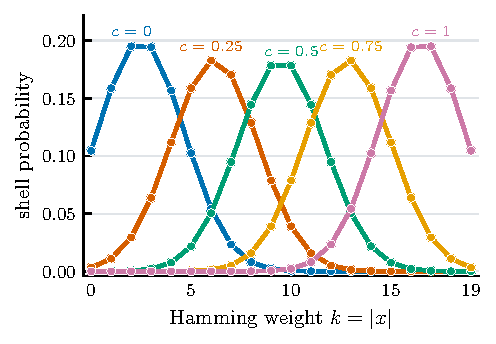
\includegraphics[width=\linewidth]{gaussian_figures/fig1_pipeline_targets.pdf}
  \end{minipage}
  \caption{State conditioning and the Gaussian target family.
  (a) Conditioning prepares a classically tractable input state $\ket{\phi(c)}$
  (a product state in the Gaussian experiment and a spin-flip two-branch state
  in the Curie--Weiss experiment); the IQP unitary and phase vector are shared
  across conditions.
  (b) Five representative 19-qubit target profiles; probability is uniform
  within each Hamming shell.
  \TODO{This is the main figure, we should either make it all about the input state conditioning or also include the Curie-Weiss dataset}}
  \label{fig:pipeline}
\end{figure*}


State conditioning therefore extends classically trained IQP Born machines from a single distribution to a condition-indexed family without reprogramming the diagonal unitary. Our evidence is limited to within-range interpolation on exchangeable targets. The Curie--Weiss experiment does not isolate the effects of the spin-flip construction and ancilla marginalization. Section~\ref{sec:universality-limit} proves that an overlap-preserving, non-multiplexed family cannot approximate every continuous conditional law. We make no claim of classical output sampling, quantum advantage, thermal-state preparation, or favorable optimization behavior \cite{shenCharacterizingTrainability2026}.


\section{Conditional IQP model}
\label{sec:model}

The conditional IQP model has two parts: a condition-dependent input state and
a condition-independent unitary. Let $G=(V,E)$ be an undirected graph with
$n=|V|$ vertices. Each vertex represents one qubit and one $R_Z$ gate, while
each edge represents an $R_{ZZ}$ gate. For
$\boldsymbol\theta\in\mathbb R^{|V|+|E|}$, the graph defines the IQP unitary
\begin{equation}
 U_{\boldsymbol\theta}=H^{\otimes n}D_G(\boldsymbol\theta)H^{\otimes n},
 \label{eq:iqp-unitary}
\end{equation}
where the diagonal layer is
\begin{equation}
 D_G(\boldsymbol\theta)=
 \left[\prod_{\{i,j\}\in E}R_{ZZ}^{(i,j)}(\theta_{ij})\right]
 \left[\prod_{i\in V}R_Z^{(i)}(\theta_i)\right].
 \label{eq:graph-diagonal}
\end{equation}
All gates in $D_G$ commute. The unitary has $|V|+|E|$ trainable parameters,
one for each vertex and edge.

For each condition $c$, an encoder prepares a state $\ket{\phi(c)}$ before the
IQP unitary. Computational-basis measurement defines
\begin{equation}
 q_{\boldsymbol\theta}(x\mid c)=
 \left|\langle x|U_{\boldsymbol\theta}|\phi(c)\rangle\right|^2,
 \qquad x\in\{0,1\}^n.
 \label{eq:cond_sampling}
\end{equation}
Equation~\eqref{eq:cond_sampling} highlights the sharing constraint:
$G$ and $\boldsymbol\theta$ are the same for every condition. The
state-preparation circuit need not have IQP form, so the full conditional
pipeline is not, in general, a strict IQP circuit. Its learned and compiled
diagonal $D_G(\boldsymbol\theta)$ remains fixed across conditions.

The state entering the diagonal layer is
$\ket{\psi(c)}=H^{\otimes n}\ket{\phi(c)}$. Classical estimation of the
Pauli-$Z$ expectation values requires samples from
$|\langle z|\psi(c)\rangle|^2$ together with ratios between computational-basis
amplitudes. This restricts the allowed encoders. Van den Nest's definition of
a computationally tractable state, which requires efficient basis sampling
and efficient amplitude evaluation, is sufficient
\cite{nestSimulatingQuantumComputers2011}. Section~\ref{sec:training} states
the weaker sampling and amplitude-ratio interface used by our estimator.

\subsection{Product-state conditioning}
The simplest way to encode the condition is a product state of single-axis rotations,
\begin{equation}
    \ket{\phi(c)}=\bigotimes_{i=1}^n R_j(\alpha_i(c))\ket{0}.
    \label{eq:product-state-encoder}
\end{equation}
Here $j\in\{X,Y\}$ denotes the rotation axis and $c\in[0,1]$ is the
normalized condition. Its physical meaning depends on the problem. The
condition changes the angles $\alpha_i(c)$ but not the IQP parameters.

%Note that the conditioning only changes $\alpha_i(c)$

\TODO{Maybe this fits better in the experimental setup section}
In our experiments we employ $R_Y$ rotations in the encoding and use the following transformation for the input,
\begin{equation}
    \alpha_i(c)=\pi(0.35-0.70c),\quad i=1,\dots,n
    \label{eq:broadcast-angle}
\end{equation}
This affine transformation is chosen heuristically to map the input interval $c \in [0, 1]$ symmetrically across the angular range $[0.35\pi, -0.35\pi]$, providing a balanced phase shift that centers the data while avoiding the periodicity bounds of the rotation gate \TODO{justify better, maybe point towards the results or do some experiment to show that this works better than simply normalizing by pi}.

Since the angle depends affinely on $c$, each output probability is a finite Fourier series whose frequencies are signed sums of the encoding frequencies \cite{schuldEffectDataEncoding2021, casasMultidimensionalFourier2023}.

\subsection{Purified product-state conditioning}
Product-state conditioning supplies one pure visible input for each condition.
To represent a condition-dependent mixed input, we extend the system with $r$
ancillas and measure only the $n$ visible qubits.


\TODO{maybe this can be reduced to an "ancilla" section as the other encoding also uses ancillas.}

Let $u\in\{0,1\}^r$ label an ancilla state and let $w_c(u)$ be a normalized
distribution. Each value of $u$ selects a visible product state
\begin{equation}
 \ket{\phi(c,u)}=
 \bigotimes_{i=1}^n R_{j_i}(\alpha_i(c,u))\ket{0}.
 \label{eq:conditional-product-branch}
\end{equation}
The joint input
\begin{equation}
 \ket{\Phi(c)}=
 \sum_{u\in\{0,1\}^r}\sqrt{w_c(u)}\ket{u}_a\ket{\phi(c,u)}_v
 \label{eq:purified-input}
\end{equation}
is a purification of the visible mixture
$\sum_u w_c(u)\ket{\phi(c,u)}\!\bra{\phi(c,u)}$. Let $N=n+r$ and let
$U_{\boldsymbol\theta}^{(N)}$ be an IQP unitary on the joint register. The
visible output distribution is
\begin{equation}
 q_{\boldsymbol\theta}(x\mid c)=
 \sum_{z\in\{0,1\}^r}
 \left|\langle x,z|U_{\boldsymbol\theta}^{(N)}|\Phi(c)\rangle\right|^2.
 \label{eq:visible-marginal}
\end{equation}
The ancillas can therefore change the rank of the visible state. If the graph
contains visible--ancilla edges, they also change the interaction structure of
the IQP unitary. These are different sources of model capacity and should be
distinguished in comparisons. Classical training remains possible only when
the joint state entering the diagonal layer supports the sampling and
amplitude-ratio operations defined in Section~\ref{sec:training}.

\subsection{Symmetry-informed conditioning}


\TODO{Simplify so its easier to understand}

Conditional models can exploit symmetries that relate different conditions,
as well as symmetries within one target distribution. Let a finite group
$\Gamma$ act on both conditions and bit strings. We want the model to satisfy
\begin{equation}
 q_\theta(g\cdot x\mid g\cdot c)=q_\theta(x\mid c),
 \qquad g\in\Gamma.
 \label{eq:conditional-equivariance}
\end{equation}
If the group does not change $c$, Eq.~\eqref{eq:conditional-equivariance}
reduces to the usual invariance $q_\theta(g\cdot x\mid c)=q_\theta(x\mid c)$.
If instead $c=h$ is a signed field and $g$ flips every bit, the same equation
becomes $q_\theta(\bar x\mid-h)=q_\theta(x\mid h)$.

Let $S_g$ implement the action on bit strings,
$S_g\ket{x}=\ket{g\cdot x}$. Equation~\eqref{eq:conditional-equivariance}
follows from two requirements:
\begin{equation}
 [U_\theta,S_g]=0,
 \qquad
 \ket{\phi(g\cdot c)}=e^{i\omega_g(c)}S_g\ket{\phi(c)}.
 \label{eq:symmetry-conditions}
\end{equation}
The first requirement makes the shared IQP unitary equivariant. The second
requires the encoder to transform conditions and output states consistently.
The phase $e^{i\omega_g(c)}$ disappears upon measurement, and hence
\begin{equation}
 \begin{aligned}
 q_\theta(g\cdot x\mid g\cdot c)
 &=\left|\langle x|S_g^\dagger U_\theta|\phi(g\cdot c)\rangle\right|^2\\
 &=\left|\langle x|U_\theta|\phi(c)\rangle\right|^2.
 \end{aligned}
 \label{eq:symmetry-proof}
\end{equation}

One way to construct such an encoder is to start from a base state
$\ket{\eta(c)}$ and average it over the joint group action,
\begin{equation}
 \ket{\phi_\Gamma(c)}=\frac{1}{\sqrt{\mathcal N(c)}}
 \sum_{g\in\Gamma}S_g\ket{\eta(g^{-1}\cdot c)},
 \label{eq:symmetrized-encoder}
\end{equation}
where $\mathcal N(c)$ normalizes the state. The group fixes how conditions and
outputs transform, while $\ket{\eta(c)}$ controls the remaining dependence on
$c$.

For a permutation $\pi$ of the qubits, the commutation requirement holds when
relabeling every qubit $i$ as $\pi(i)$ leaves the diagonal layer unchanged.
Concretely, $\{i,j\}\in E$ if and only if
$\{\pi(i),\pi(j)\}\in E$, and gates mapped into one another use the same
angles: $\theta_i=\theta_{\pi(i)}$ and
$\theta_{ij}=\theta_{\pi(i)\pi(j)}$. Every permutation preserves the edge set
of a complete graph. The corresponding unitary is invariant under all qubit
permutations when all vertex angles are equal and all edge angles are equal.

Symmetry does not imply classical tractability. Even if the base state
$\ket{\eta(c)}$ is easy to prepare, the coherent sum in
Eq.~\eqref{eq:symmetrized-encoder} may be hard to sample or query. A useful
case occurs when the amplitudes depend only on a polynomial number of classes,
such as the $n+1$ Hamming-weight values. One can then sample the class first
and evaluate amplitude ratios from the classes of $z$ and $z\oplus a$.

\section{Limits of conditional universality}
\label{sec:universality-limit}

Classical tractability controls access to the estimator, not conditional
expressivity. Let $\rho_c$ be the input density operator on every visible,
hidden, and ancillary qubit. For fixed parameters $\theta$, the IQP unitary,
partial trace, and visible measurement define a quantum-to-classical channel
$\mathcal M_\theta$, so
$q_\theta(\cdot\mid c)=\mathcal M_\theta(\rho_c)$. Write
$D_{\rm tr}(\rho,\sigma)=\frac12\lVert\rho-\sigma\rVert_1$.

\begin{proposition}[Pairwise distinguishability bound]
\label{prop:main-pairwise-bound}
For any target conditional law $p$ and any two conditions $c,c'$,
\begin{multline}
 \sup_t\TVD\!\left(q_\theta(\cdot\mid t),p(\cdot\mid t)\right)\\
 \geq\frac12\left[
 \TVD\!\left(p(\cdot\mid c),p(\cdot\mid c')\right)
 -D_{\rm tr}(\rho_c,\rho_{c'})
 \right]_+ ,
 \label{eq:main-pairwise-bound}
\end{multline}
where $[u]_+=\max\{u,0\}$.
\end{proposition}

Measurement cannot increase trace distance. Combining this contraction with
the triangle inequality proves Proposition~\ref{prop:main-pairwise-bound};
Appendix~\ref{app:conditional-universality} gives the full derivation. An
exactly universal conditional family must represent target laws with disjoint
support at any chosen pair of conditions. Equation~\eqref{eq:main-pairwise-bound}
then requires $D_{\rm tr}(\rho_c,\rho_{c'})=1$ for every $c\neq c'$, which is
equivalent to orthogonal input supports.

The same obstruction survives resource scaling. We call an encoder family
overlap preserving, and hence non-multiplexed, if some $c\neq c'$ and
$\gamma>0$ satisfy
\begin{equation}
 D_{\rm tr}\!\left(\rho_c^{(R)},\rho_{c'}^{(R)}\right)
 \leq1-\gamma
 \quad\text{for every allowed resource }R.
 \label{eq:main-overlap-preserving}
\end{equation}
A total-variation-continuous target can interpolate from
$\delta_{0^n}$ at $c$ to $\delta_{1^n}$ at $c'$. Every model in the family
then has uniform error at least $\gamma/2$. Thus universal approximation of
all continuous conditional laws forces every distinct pair of condition
states to become asymptotically perfectly distinguishable. Such states are
operational labels in the limit: their discrimination error tends to zero,
enabling asymptotically reliable condition routing.

Coherent selector notation does not remove this routing structure. If a
factorized selector state $\sigma_S(c)$ controls a joint IQP diagonal
$D=\sum_s\ket{s}\!\bra{s}\otimes D_s$ and $S$ is discarded, then
\begin{equation}
 q(x\mid c)=\sum_s
 \langle s|\sigma_S(c)|s\rangle q_s(x).
 \label{eq:main-selector-mixture}
\end{equation}
The off-diagonal selector coherences vanish under the partial trace.
Selector and Bernstein constructions therefore produce a classical mixture
of condition-independent IQP branches rather than a shared universal
conditional mechanism.

For the broadcast product encoder with $N$ copies of
$R_Y(\alpha(c))\ket{0}$, the input trace distance is
\begin{equation}
 d_N(c,c')=
 \sqrt{1-\cos^{2N}\!\left(
 \frac{\alpha(c)-\alpha(c')}{2}\right)}.
 \label{eq:main-broadcast-distance}
\end{equation}
If $\alpha$ is $L_\alpha$-Lipschitz, a continuous target that changes between
two deterministic strings over an interval of width $h$ has uniform error at
least
\begin{equation}
 \frac12\left(1-\frac{\sqrt N L_\alpha h}{2}\right)_+.
 \label{eq:main-ramp-bound}
\end{equation}
At the Gaussian setting $N=19$, $L_\alpha=0.70\pi$, and $h=0.01$, this
certificate equals $0.4760$. It is a worst-case expressivity result, not a
bound on the reported Gaussian targets. Fixed Fourier bandwidth and parameter
dimension impose separate restrictions. In particular, the complete
two-local models have 190 phases versus $5(2^{19}-1)=2{,}621{,}435$
conditional-table dimensions in the five-condition Gaussian setting, and 91
phases versus $6(2^8-1)=1{,}530$ dimensions at the six Curie--Weiss training
temperatures. Appendix~\ref{app:conditional-universality} proves each claim
and states the narrower compatibility condition left open by this no-go
result.

\section{Conditional IQP training}
\label{sec:training}

For training we employ the maximum mean discrepancy (MMD) loss \cite{grettonKernelTwoSample2012} adapted to the conditional generation setting. The MMD is an integral probability metric defined by a positive-definite kernel $k$. For two distributions $p$ and $q$ on $\bits^n$, the squared MMD is
\begin{equation}
\begin{aligned}
\mmd^2(p,q)={}&\E_{x,x'\sim p}[k(x,x')]
  -2\E_{x\sim p,\,y\sim q}[k(x,y)]\\
  &+\E_{y,y'\sim q}[k(y,y')].
\end{aligned}
\label{eq:mmd-population}
\end{equation}

We use the Gaussian kernel, which for binary strings is
\begin{equation}
 k_\sigma(x,y)=\exp[-d_H(x,y)/(2\sigma^2)],
 \label{eq:hamming-kernel}
\end{equation}
where $d_H$ is the Hamming distance. Let $a\in\{0,1\}^n$ have independent
coordinates
\begin{equation}
 a_i\sim\operatorname{Bernoulli}(q_\sigma),
 \qquad q_\sigma=\frac{1-e^{-1/(2\sigma^2)}}{2}.
 \label{eq:mask-distribution}
\end{equation}
Writing $\chi_a(x)=(-1)^{a\cdot x}$, the kernel has the character
representation
\begin{equation}
 k_\sigma(x,y)=\E_a[\chi_a(x)\chi_a(y)].
 \label{eq:kernel-character}
\end{equation}
Define the character moment of a distribution $p$ by
$\mu_p(a)=\E_{x\sim p}[\chi_a(x)]$. Substituting
Eq.~\eqref{eq:kernel-character} into Eq.~\eqref{eq:mmd-population} gives
\begin{equation}
 \mmd_\sigma^2(p,q)=
 \E_a\left[(\mu_p(a)-\mu_q(a))^2\right].
 \label{eq:mmd-character}
\end{equation}
For a Born machine, $\mu_q(a)$ is the expectation value of the Pauli string
$Z_a=\bigotimes_i Z_i^{a_i}$. The MMD can therefore be estimated by sampling
Pauli-$Z$ moments rather than bit strings from the model.

The training objective balances the per-condition losses equally over the training conditions $C$,
\begin{equation}
\mathcal{L}(\theta)=\frac{1}{|C|}\sum_{c\in C}\frac{1}{|\Sigma|}
\sum_{\sigma\in\Sigma}\mmd^2_\sigma\!\bigl(p(\cdot\mid c),\,
q_\theta(\cdot\mid c)\bigr).
\label{eq:conditional-objective}
\end{equation}

We next state the classical estimator for these moments. Let
\begin{equation}
 \psi_c(z)=\langle z|H^{\otimes n}|\phi(c)\rangle
 \label{eq:reference-amplitude}
\end{equation}
be the computational-basis amplitudes of the state entering $D_G$. The
encoder is admissible when, uniformly over $c$, a classical algorithm can
sample $z$ from $|\psi_c(z)|^2$ and evaluate
\begin{equation}
 R_c(z,a)=\frac{\psi_c(z\oplus a)}{\psi_c(z)}
 \label{eq:amplitude-ratio}
\end{equation}
for sampled $z$ and every mask $a$ used by the loss. The ratio need only be
defined on the support of $|\psi_c|^2$. A sampler without amplitude-ratio
access is not sufficient.

Let $f_{\boldsymbol\theta}(z)$ be the phase defined by
$D_G(\boldsymbol\theta)\ket{z}=e^{if_{\boldsymbol\theta}(z)}\ket{z}$ and set
\begin{equation}
 \Delta f_{\boldsymbol\theta}(z,a)=
 f_{\boldsymbol\theta}(z\oplus a)-f_{\boldsymbol\theta}(z).
\end{equation}
Conjugating $Z_a$ through the final Hadamards gives $X_a$, and hence
\begin{equation}
 \begin{aligned}
 \mu_{q_{\boldsymbol\theta}}(a\mid c)
 &=\langle\psi(c)|D_G^\dagger X_aD_G|\psi(c)\rangle\\
 &=\operatorname{Re}\E_{z\sim|\psi_c|^2}
 \left[R_c(z,a)e^{i\Delta f_{\boldsymbol\theta}(z,a)}\right].
 \end{aligned}
 \label{eq:pauli-estimator}
\end{equation}
The phase difference is computed directly from the gates in $D_G$, with cost
linear in $|V|+|E|$. Product-state encoders provide the required samples and
ratios by factorizing over qubits. Other encoders are allowed when they expose
the same two operations.

The square in Eq.~\eqref{eq:mmd-character} must be estimated without squaring
a single noisy sample mean. For a fixed condition, bandwidth, and mask, let
\begin{equation}
 Y_s=\chi_a(x_s)-
 \operatorname{Re}\left[R_c(z_s,a)
 e^{i\Delta f_{\boldsymbol\theta}(z_s,a)}\right],
\end{equation}
where $x_s\sim p(\cdot\mid c)$ and
$z_s\sim|\psi_c|^2$ are independent. Then
$\E[Y_s]=\mu_p(a\mid c)-\mu_{q_{\boldsymbol\theta}}(a\mid c)$, and the
U-statistic
\begin{equation}
 \widehat{\Delta^2}(a,c)=
 \frac{1}{S(S-1)}\sum_{s\ne t}Y_sY_t
 \label{eq:mmd-u-statistic}
\end{equation}
is unbiased for the squared moment discrepancy. Sampling $c$, $\sigma$, and
$a$ according to Eqs.~\eqref{eq:conditional-objective} and
\eqref{eq:mask-distribution} gives an unbiased finite-sample estimate of the
conditional loss.

The encoder maps are fixed during this optimization, so
$|\psi_c(z)|^2$ and $R_c(z,a)$ do not depend on $\boldsymbol\theta$.
Gradients with respect to the IQP phases follow by differentiating only
$\Delta f_{\boldsymbol\theta}$ in the sampled expression. If the encoder
contains trainable parameters that change its sampling distribution, this
argument no longer applies without an additional gradient estimator.

The amplitude ratio also gives a simple second-moment bound,
\begin{equation}
 \E_{z\sim|\psi_c|^2}\left[|R_c(z,a)|^2\right]
 =\sum_{z:\psi_c(z)\ne0}|\psi_c(z\oplus a)|^2\leq1.
 \label{eq:ratio-second-moment}
\end{equation}
The single-sample Pauli estimator therefore has variance at most one. This is
not a zero-variance result and does not guarantee favorable optimization.
For an ancilla model, the same derivation applies to the joint state. Visible
masks are padded with zeros on the unmeasured ancillas.

Classical trainability in this work refers only to estimating the observables,
loss, and phase gradients. It does not provide efficient classical samples
from $q_{\boldsymbol\theta}(x\mid c)$ or efficient exact evaluation of its
probabilities.

\section{Experimental setup}
\label{sec:experiments}

\subsection{Research questions and confirmation policy}

The experiments address four questions. First, can one fixed IQP unitary model
a family of distributions when only its input state depends on the condition?
Second, does the learned response interpolate to conditions excluded from
training and checkpoint selection? Third, which part of an ancilla-assisted
construction supplies useful capacity: the rank of the visible input, the
visible--ancilla interactions, or the additional trainable phases? Finally,
can an equivariant encoder transfer information between conditions related by
a known symmetry?

We separated model development from confirmation. Earlier runs were used to
select the encoder families, condition maps, optimization schedule, and
ancilla counts. We then froze the protocols below and assigned new data and
optimizer seeds to every confirmatory fit. We report every declared run,
including negative and mixed comparisons. All conditions called held out lie
strictly inside the training interval; we therefore use \emph{interpolation}
rather than extrapolation throughout.

\subsection{Target families and condition splits}

The first target is a discrete Gaussian over the Hamming weight
$K(x)=\sum_i x_i$. For condition $c\in[0,1]$, the target mean is
$\mu(c)=n(0.15+0.70c)$ and the nominal width is $w\sqrt n$. We calibrate the
location of the truncated Gaussian on $K\in\{0,\ldots,n\}$ so that its mean is
exactly $\mu(c)$, then distribute the shell probability uniformly over the
$\binom nk$ strings of weight $k$. The factorial study uses

\begin{equation}
\begin{split}
 n&\in\{8,12,16,19\},\qquad
 w\in\{0.35,0.50,0.75\},\\
 C_{\mathrm{train}}&=\{0,0.25,0.50,0.75,1\},\\
 C_{\mathrm{test}}&=\{(2j+1)/16:j=0,\ldots,7\}.
\end{split}
\label{eq:gaussian-grids}
\end{equation}
At $n=19$ and $w=0.50$, we also use nested grids containing
$K\in\{2,3,5,9\}$ training conditions. One allocation keeps 10,000 training
and 2,000 validation strings per condition. The other divides fixed totals of
18,000 and 3,600 strings among the $K$ conditions.

The second target is the finite Curie--Weiss law
\begin{equation}
 \begin{aligned}
 p_{\beta,h}(x)&=\frac{1}{Z(\beta,h)}
 \exp\left[\frac{\beta}{2n}M(x)^2+hM(x)\right],\\
 M(x)&=\sum_{i=1}^n(2x_i-1).
 \end{aligned}
 \label{eq:curie-weiss-target}
\end{equation}
The temperature study sets $h=0$, uses $n\in\{8,12,16\}$, trains at
$\beta\in\{0.5,0.7,0.9,1.1,1.3,1.5\}$, and evaluates at the interleaved
temperatures $\{0.6,0.8,1.0,1.2,1.4\}$. The ancilla mechanism comparison
focuses on the critical region $\beta\in\{0.8,1.0,1.2\}$ but reports the full
temperature curve. A separate field study fixes $\beta=1$, trains at
$h\in\{0,0.15,0.30\}$, and tests at $h=\pm0.075$ and $\pm0.225$. Reflected
training fields $-0.15$ and $-0.30$ test symmetry transfer without adding
negative-field samples to the one-sided training set.

The applied benchmark uses the public Muonic Force Carrier event samples at
incoming energies $E\in\{50,75,100,125,150,175,200\}$ GeV
\cite{kissConditionalBornMachine2022}. We discretize the scaled outgoing-muon
energy into 16, 32, and 64 bins and encode the bin index using either ordinary
binary or fixed Gray coding. For each representation, 10,000 events per
observed energy form the training set, 2,000 form the validation set, and the
remaining events are reserved for final evaluation. Five folds omit one
interior energy in turn, $E\in\{75,100,125,150,175\}$ GeV. Before conditional
training, three development seeds screen independent fits at 50, 125, and
200 GeV. We continue a coding--resolution cell only if every anchor has median
validation TVD at most $0.10$ and no seed exceeds $0.15$. Failed screens remain
part of the reported experiment.

\subsection{Models and controls}

Unless stated otherwise, the IQP diagonal contains one $R_Z$ gate per qubit
and one $R_{ZZ}$ gate per edge of the complete graph. A model on $N$ qubits
therefore has $N(N+1)/2$ trainable phases. The Gaussian and MFC conditioned
models use the product-state encoder in Eq.~\eqref{eq:product-state-encoder}
with the affine map in Eq.~\eqref{eq:broadcast-angle}. Their no-condition
controls receive the neutral input $c=1/2$ for every target while retaining
the same circuit, data, and optimization budget. Independent single-condition
circuits provide a capacity reference. At a held-out Gaussian condition we
also compare against the better adjacent stored output and against the
target-blind barycentric mixture of the two adjacent outputs.
For MFC, the separate circuit is an oracle capacity reference fitted to the
omitted energy's training split; it is excluded from held-out-condition
generalization claims.

For the zero-field Curie--Weiss family, the $m=0$ controls use either the
product input or the fixed spin-flip two-branch input. The ancilla study adds
$r\in\{1,3,5\}$ qubits and compares three constructions at every visible size.
The \emph{full} model uses the complete graph on all $n+r$ qubits. The
\emph{disconnected} model uses the same purified input but removes every
visible--ancilla edge, which isolates the effect of the visible input rank.
The \emph{matched visible} control removes the ancillas and adds a fixed set
of distinct three-qubit diagonal generators until its phase count equals that
of the full model. These three-local terms are used only as a capacity control;
they are not part of the graph ansatz defined in Section~\ref{sec:model}.
No-condition controls are evaluated at $r=0$ and $r=5$.

For the field experiment, let
\begin{equation}
 \ket{\eta(h)}=
 \bigotimes_{i=1}^nR_Y[-7\pi h/6]\ket{0}.
\end{equation}
The symmetry-informed model uses
\begin{equation}
 \ket{\phi_{\mathrm{eq}}(h)}=
 \frac{\ket{\eta(h)}+X^{\otimes n}\ket{\eta(-h)}}
 {\sqrt{\mathcal N(h)}}.
 \label{eq:field-equivariant-encoder}
\end{equation}
It obeys
$\ket{\phi_{\mathrm{eq}}(-h)}=X^{\otimes n}
\ket{\phi_{\mathrm{eq}}(h)}$ and hence enforces
$q_\theta(\bar x\mid-h)=q_\theta(x\mid h)$. We compare it with an
unconstrained product encoder trained on the same nonnegative fields, the same
product encoder trained on both signs, and a spin-flip-invariant encoder that
incorrectly imposes $q(x\mid h)=q(\bar x\mid h)$ at nonzero field.

The MFC benchmark adds two classical references. Linear interpolation between
the adjacent empirical training histograms gives a target-blind nonparametric
baseline. A categorical neural network takes the normalized incoming energy
as input, applies two width-32 hidden layers, and predicts the bin
probabilities with a softmax output. We treat these as contextual references,
not as targets that the IQP model must outperform.

\subsection{Training and evaluation}

All IQP fits optimize only the condition-independent phases
$\boldsymbol\theta$; the encoder maps remain fixed. We use Adam for 2,000
updates with cosine learning-rate decay from $10^{-2}$ to $10^{-3}$. The loss
averages the Hamming kernels with $\sigma\in\{1,2,4\}$. Each training estimate
uses 64 character masks and 8,192 reference samples per bandwidth. Every 25
updates, a fixed validation estimate with 256 masks and 16,384 reference
samples selects the checkpoint with the lowest conditional MMD. Held-out
conditions and final target probabilities never enter checkpoint selection.
The categorical MFC baseline minimizes cross entropy under the same
training--validation split and selects its checkpoint by validation loss.

For the synthetic targets, exact enumeration after checkpoint selection gives
the bitstring TVD, Hamming-profile TVD, conditional moments, and exact MMD. For
an ancilla model we first sum the joint probabilities over the unmeasured
qubits. The MFC evaluation decodes the predicted bit strings to energy bins and
reports TVD, one-dimensional Wasserstein distance, and errors in the first two
scaled-energy moments. The field study also reports the equivariance defect
\begin{equation}
 \epsilon_{\mathrm{eq}}(h)=\frac12\sum_x
 \left|q_\theta(x\mid h)-q_\theta(\bar x\mid-h)\right|.
 \label{eq:equivariance-defect}
\end{equation}
The supplementary estimator audit compares moments, losses, and gradients
against exact calculations at sample budgets
$S\in\{256,1024,4096,16384\}$. A separate topology ablation compares complete,
rectangular-grid, and heavy-hex graphs at $n=19$, $w=0.50$, and five training
conditions.

\subsection{Statistical analysis}

The confirmatory campaign uses ten fresh optimizer seeds, numbered 100
through 109, with matched data draws wherever targets are sampled. We report
the median and interquartile range across
seeds. Method effects are computed within each seed after averaging over the
declared conditions, then summarized by a deterministic paired bootstrap with
10,000 resamples and a 95\% interval. The seed, rather than an individual
condition or bit string, is the replication unit. These are cellwise intervals;
the frozen protocol does not apply a familywise correction across contrasts.

For Gaussian interpolation, we require the conditioned model to improve on
the no-condition control at held-out conditions and allow at most $0.05$ added
TVD relative to the interior training conditions. The adjacent lookup and
mixture comparisons are reported without a required win. The ancilla analysis
tests the three paired differences identified above rather than combining them
into one effect. The equivariant field model must improve on one-sided
unconstrained training at negative fields and remain within $0.02$ TVD of the
two-sided model. For MFC data, the generalization claim is restricted to the
comparison with the no-condition IQP control. We make no empirical claim about
extrapolation, efficient classical output sampling, or quantum advantage.


\section{Results}

\TODO{Insert the Gaussian confirmatory results before the Curie--Weiss
subsection.}

\subsection{Ancilla-assisted Curie--Weiss interpolation}

In the tested ladder, the full ancilla model interpolates across the finite
Curie--Weiss crossover once the ancilla register contains at least three
qubits. At the three
held-out temperatures nearest the transition, the $r=5$ model attains median
profile TVDs of $0.051$, $0.058$, and $0.069$ for $n=8$, $12$, and $16$,
respectively. The corresponding bitstring TVDs are $0.075$, $0.098$, and
$0.132$. Thus the model retains the magnetization profile as the visible
system grows, although its error on individual bit strings increases more
strongly with size.

Conditioning accounts for most of this accuracy. The $r=5$ no-condition
control has the same generator count and optimization budget but receives the
neutral input at every temperature. Its median critical-region profile TVD
increases from $0.117$ at $n=8$ to $0.198$ at $n=16$, compared with $0.051$ to
$0.069$ for the conditioned model. Bitstring TVD separates the models more
sharply at the two larger sizes: the conditioned and no-condition values are
$0.098$ versus $0.236$ at $n=12$, and $0.132$ versus $0.312$ at $n=16$.
The same ordering holds when all five held-out temperatures are included.
% TODO: Replace numerical literals with generated macros after adding the
% paired conditioned-versus-no-condition contrast to the finalizer.

The interpolation error is not uniform in temperature. For the $n=16$,
$r=5$ model, median profile TVD is $0.058$, $0.038$, and $0.117$ at the
held-out temperatures $\beta=0.8$, $1.0$, and $1.2$. The model therefore
represents the central held-out point accurately but overshoots the growth of
the ordered modes on the colder side of the crossover. The same pattern is
visible in the magnetization and susceptibility: both follow the target
response, but their largest critical-region bias occurs at $\beta=1.2$ and
grows with $n$. These finite systems test interpolation through a crossover;
they do not estimate a critical exponent or the thermodynamic critical point.

The paired mechanism comparisons explain why the larger ancilla models work.
Relative to the spin-flip $m=0$ model, the disconnected construction improves
bitstring TVD at every size and ancilla count. The corresponding profile-TVD
effect is also positive except for the inconclusive $n=16$, $r=1$ cell. Once
$r\geq3$, restoring visible--ancilla interactions improves both metrics in
all twelve combinations of size, ancilla count, and metric. At $r=5$, the
profile-TVD
effects range from $0.024$ to $0.027$, while the bitstring-TVD effects range
from $0.061$ to $0.087$. The full model also beats the parameter-matched
visible control for both metrics at $r=3$ and $r=5$. Hence neither additional
phases alone nor a mixed visible input without cross-register interactions
accounts for the full result.

The $r=1$ cells give a useful boundary rather than a smaller version of the
same effect. Adding visible--ancilla interactions to the disconnected $r=1$
model worsens profile TVD at all three sizes. Against the parameter-matched
visible model, the full $r=1$ model improves bitstring TVD but worsens profile
TVD at $n=8$ and $n=12$ and gives an inconclusive profile difference at
$n=16$. In this comparison, the single-ancilla model redistributes probability
among individual strings without improving the magnetization-shell
probabilities.
The confirmatory evidence supports the combined $r=3$ and $r=5$
construction, not a monotone claim that every added ancilla or interaction is
beneficial.

\section{Discussion}
Conditional generation with IQP Born machines represents a promising avenue for quantum generative modeling as it combines the scalability of IQP circuits and the utility of more general models that enable conditional generation...

\section{Conclusions}
The main contribution of this work is the conditional formulation of classically trained IQP Born machines. The contraction result fixes the scope of this formulation: a non-multiplexed encoder cannot be universal for every continuous conditional law. A positive approximation theorem must instead restrict the target family to distributions whose pairwise total-variation geometry is compatible with the trace-distance geometry of the input encoding. %The proposed framework leverages previous literature on computationally tractable states and reformulates the MMD for the conditional generation case to


\section*{DATA AVAILABILITY}
The code and data supporting the findings of this study are openly available in Zenodo \cite{???}.

\section*{Acknowledgments}
OB is a fellow of Eurecat’s ``Vicente L\'opez'' PhD grant program. This piece of research was carried out with the partial support of the following granted projects: $\cdots$.

\bibliographystyle{apsrev4-2}
\bibliography{references}

\clearpage
\onecolumngrid
\appendix
\section{Analytical details}
\label{app:analysis}

\subsection{Finite conditional response}

Let the product-state angle map be affine,
$\alpha(c)=b+Wc$, where row $i$ of $W$ is $w_i^{\mathsf T}$. Expanding each
local sine and cosine into exponentials shows that every amplitude has
frequencies in signed sums of the rows of $W$. Squaring an amplitude gives
\begin{equation}
 \Omega_{\mathrm{full}}(W)
 \subseteq
 \left\{\sum_{i=1}^{n}s_iw_i:s_i\in\{-1,0,1\}\right\}.
\end{equation}
Coincident frequencies and vanishing coefficients can make the inclusion
strict. The argument establishes a finite response space at fixed encoding
width; it does not provide an efficient coefficient-evaluation procedure or a
universal-approximation result.

For an observable $Z_a$, the active-generator expansion retains only
generators with $a\cdot g_j=1\pmod 2$. Grouping active subsets by their XOR
mask $h$ and using $\langle Y_i\rangle=0$ for a real $R_Y$ product input
removes terms with $h\wedge a\ne0$. Observable responses can therefore have
strictly smaller frequency support than full probabilities. This is a direct
specialization of established circuit-Fourier and IQP active-generator
descriptions
\cite{schuldEffectDataEncoding2021,casasMultidimensionalFourier2023,
recio-armengolTrainClassicalDeploy2026}.

\subsection{Product and block-product estimator}

Write the tractable reference amplitude as
$\phi_c(z)=\langle z|H^{\otimes n}|\phi(c)\rangle$. The classical
observable estimator samples $z$ from $|\phi_c(z)|^2$ and evaluates an
amplitude ratio $R_c(z,a)=\phi_c(z\oplus a)/\phi_c(z)$ together with the
phase factor generated by the active diagonal terms. The ratio obeys
\begin{align}
 \E_z|R_c(z,a)|^2
 &=\sum_{z:|\phi_c(z)|>0}|\phi_c(z)|^2
   \frac{|\phi_c(z\oplus a)|^2}{|\phi_c(z)|^2} \\
 &\leq \sum_z|\phi_c(z\oplus a)|^2=1.
\end{align}
The equality used in the main text holds when the shifted support is fully
covered; the inequality is the general statement when some reference
amplitudes vanish. In either case the variance is at most one. The bound is on
the estimator variance, not on optimizer convergence or raw gradient
magnitude.

The same argument applies to a block-product input
$|\phi(c)\rangle=\bigotimes_B|\phi_B(c)\rangle$. The ratio factorizes over
blocks, and normalization gives
\begin{equation}
 \E|R_c(z,a)|^2
 \leq\prod_B\sum_{z_B}|\phi_B(z_B\oplus a_B)|^2=1.
\end{equation}
This observation supports the archived block-encoding study in
Sec.~\ref{app:encoding}. The Gaussian production experiments use single-qubit
product states, while the Curie--Weiss production experiments use the
spin-flip two-branch state, whose radial amplitude also factorizes over
Hamming shells and is classically tractable.

\subsection{Hamming-kernel character loss}

For $a_i\sim\operatorname{Bernoulli}(q_\sigma)$ with $q_\sigma$ defined in
Eq.~\eqref{eq:mask-law},
\begin{align}
 \E_a[(-1)^{a\cdot(x\oplus y)}]
 &=\prod_i\bigl[(1-q_\sigma)+q_\sigma(-1)^{x_i\oplus y_i}\bigr]\\
 &=\exp[-d_H(x,y)/(2\sigma^2)].
\end{align}
For condition set $C$, the training objective is the balanced average
\begin{equation}
 \mathcal L(\theta)=\frac{1}{|C|}\sum_{c\in C}
 \mmd^2(q_\theta(\cdot\mid c),p(\cdot\mid c)).
\end{equation}
Independent model and target draws give the standard unbiased U-statistic.
All random streams for masks, model samples, target batches, and validation
are derived separately and recorded in the campaign artifacts.

\section{Gaussian protocol and complete factorial summary}
\label{app:gaussian-protocol}

For each $n$, width factor $s$, and condition $c$, the target shell law is a
truncated discrete Gaussian. Its untruncated location is calibrated so that
the truncated mean is exactly $n(0.15+0.70c)$, and its nominal width is
$s\sqrt n$. Conditional and no-condition models share the complete two-local
generator bank, initialization, datasets, optimizer seed, minibatches, and
estimator streams. Single-condition references use condition-tagged streams.

The factorial contains $4\times3\times10$ seed cells and 840 atomic fits.
The condition-count study adds 180 fits for a total of 1,020. Training uses
10,000 strings and validation uses 2,000 strings per condition in the
fixed-per-condition regime. The fixed-total regime divides 18,000 training and
3,600 validation strings across conditions using prefixes of the same master
pools. Held-out conditions have no sample role in the stored datasets.

Table~\ref{tab:factorial-all} reports every size--width profile-TVD effect.
Positive no-condition effects favor conditioning. Positive adjacent-reference
or mixture effects would favor the shared model.

\begin{table*}[t]
\centering
\scriptsize
\caption{Gaussian factorial profile-TVD effects with paired 95\% bootstrap
intervals. Status letters are S for supported, M for mixed, and U for
unsupported, in the order no-condition, adjacent-reference, mixture.}
\label{tab:factorial-all}
\begin{tabular}{@{}rrp{0.21\textwidth}p{0.21\textwidth}
  p{0.21\textwidth}l@{}}
\toprule
$n$ & $s$ & no condition $-$ conditioned &
adjacent reference $-$ conditioned &
mixture $-$ conditioned & status\\
\midrule
\tableinput{generated/factorial_cells.tex}
\bottomrule
\end{tabular}
\end{table*}

Table~\ref{tab:condition-count-compact} shows the condition-density result
used in the main text. The full per-condition rows, worst-condition values,
paired intervals, and exact probability vectors remain in the machine-readable
report.

\begin{table*}[t]
\centering
\small
\caption{Condition-count study at $n=19,s=0.50$. Mean and worst are held-out
profile TVD. The shared model keeps 190 phases and 2,000 updates.}
\label{tab:condition-count-compact}
\resizebox{\textwidth}{!}{%
\begin{tabular}{rlllrrrrr}
\toprule
$K$ & regime & train/condition & validation/condition & mean & worst &
phases & shared updates & reference updates\\
\midrule
\tableinput{generated/condition_count_cells.tex}
\bottomrule
\end{tabular}}
\end{table*}

Profile TVD intentionally quotients out within-shell variation. The exact
raw-bitstring report shows that low profile error does not imply a uniform law
inside each shell. We retain the raw probabilities and all secondary metrics in
the release artifacts rather than reproducing hundreds of diagnostic rows in
the PDF.

\section{Curie--Weiss protocol and results}
\label{app:curie-protocol}

For $s_i=2x_i-1$, $M=\sum_i s_i$, and $n=8$, the exact target is
\begin{equation}
 p_\beta(x)=Z_\beta^{-1}\exp\!\left(\frac{\beta M^2}{2n}\right).
\end{equation}
The campaign checks normalization, permutation invariance, and spin-flip
invariance before writing a dataset. Each of ten dataset archives contains
10,000 training and 2,000 validation strings at the six training
temperatures. Exact laws at held-out midpoints enter only after checkpoint
selection.

The v3 broadcast map is piecewise linear. Its knots were chosen from
development screens before production and are recorded in the manifest. The
map is not presented as target-independent. The production model uses the
spin-flip two-branch state on eight visible and five ancilla inputs, applies a
complete two-local 13-qubit IQP unitary, and sums the exact joint law over all
ancilla outcomes. The encoding family and map were frozen before the 80
production fits.

Table~\ref{tab:cw-effects} gives the complete aggregate comparison set.
Temperatures are averaged within seed before bootstrapping. Positive effects
favor the named conditioned model. The shared model matches the adjacent
mixture and improves on the target-aware adjacent oracle in this campaign;
both profile and raw TVD improve relative to no conditioning.

\begin{table*}[t]
\centering
\scriptsize
\caption{All paired Curie--Weiss v3 effects.}
\label{tab:cw-effects}
\begin{tabular}{p{0.62\textwidth}cc}
\toprule
comparison & effect [95\% interval] & status\\
\midrule
\curieweissancillaeffects
\bottomrule
\end{tabular}
\end{table*}

The five-ancilla choice followed a separate three-seed development study at
$r\in\{0,1,3\}$. It motivated adding latent capacity but did not test
$r=5$, establish an optimal ancilla count, or isolate mixed-state rank from
parameter count.

\begin{table}[t]
\centering
\caption{Ancilla development study. Entries are mean held-out TVD.}
\label{tab:cw-ancilla-pilot}
\begin{tabular}{rrcc}
\toprule
$r$ & model & profile TVD & raw TVD\\
\midrule
\curieweissancillapilot
\bottomrule
\end{tabular}
\end{table}

\subsection{Historical v2 matched-capacity diagnostic}

This diagnostic predates the v3 spin-flip campaign. It compares the v2
product-input ancilla model with a visible-only model containing every
nonempty one-, two-, and three-qubit diagonal generator on eight visible
qubits:
\begin{equation}
 \binom81+\binom82+\binom83=8+28+56=92.
\end{equation}
This is one phase more than the five-ancilla complete two-local model. The
control reuses the v2 datasets, product-input angle map, support-hashed
initialization, estimator streams, 2,000-step optimizer, validation checkpoint
rule, and exact evaluation grid. It does not reuse the v3 input state and is
therefore neither a capacity match for v3 nor evidence that ancillas cause the
v3 improvement. Critical aggregates average
$\beta\in\{0.9,1.0,1.1\}$; cold aggregates average
$\beta\in\{1.3,1.4,1.5\}$.

\ifcapacitycontrolresults
\begin{table}[t]
\centering
\caption{Matched-capacity paired effects. Positive values mean lower TVD for
the five-ancilla model.}
\label{tab:capacity-effects}
\begin{tabular}{lcc}
\toprule
region & profile TVD & raw TVD\\
\midrule
held out & \CapacityProfileHeldOut{} & \CapacityRawHeldOut{}\\
critical & \CapacityProfileCritical{} & \CapacityRawCritical{}\\
cold & \CapacityProfileCold{} & \CapacityRawCold{}\\
\bottomrule
\end{tabular}
\end{table}
\fi

\begin{figure}[H]
\centering
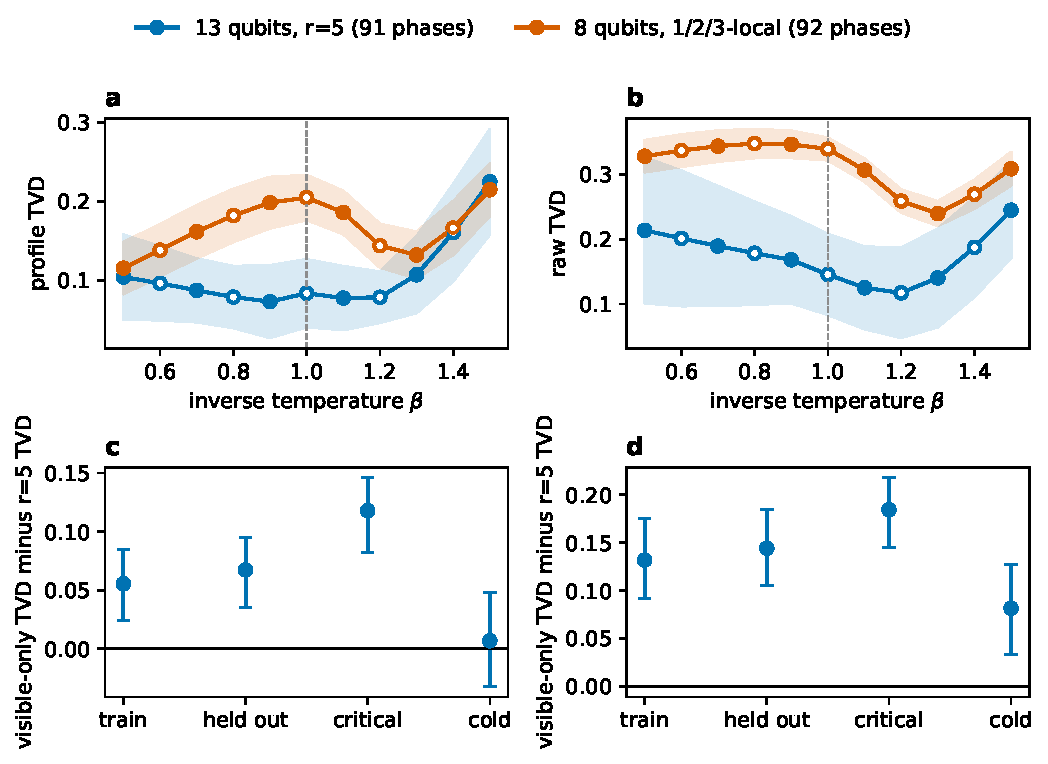
\includegraphics[width=\textwidth]{curie_weiss_ancilla_figures/matched_capacity_v2.pdf}
\caption{Historical v2 matched-capacity diagnostic. Mean profile and raw TVD
and paired regional effects compare the 91-phase v2 product-input ancilla
model with the 92-phase visible-only model. Positive effects favor the v2
ancilla model. This is not a matched control for the v3 spin-flip model.}
\label{fig:capacity-control}
\end{figure}

\section{Exploratory symmetry screens}
\label{app:symmetry-screens}

These post-core screens test whether matching an input state's symmetry to a
target can improve finite-system fits. They were designed after the core
campaigns and are not confirmatory evidence for the v3 result.

\paragraph{Two-block $Z_2^2$.} A two-block Curie--Weiss target
$p(s)\propto\exp[\beta(M_A^2+M_B^2)/16]$ on two eight-spin blocks is invariant
under independently flipping each block. The tested input is a product of two
two-branch states,
$|\phi\rangle=(|p_A\rangle^{\otimes8}+X^{\otimes8}|p_A\rangle^{\otimes8})
\otimes(|p_B\rangle^{\otimes8}+X^{\otimes8}|p_B\rangle^{\otimes8})$.
Across ten matched seeds it outperforms the product and single-$Z_2$ inputs on
the reported held-out metrics. This ordering is a screen result, not a general
theorem about symmetry-matched encodings.

\begin{figure}[H]
\centering
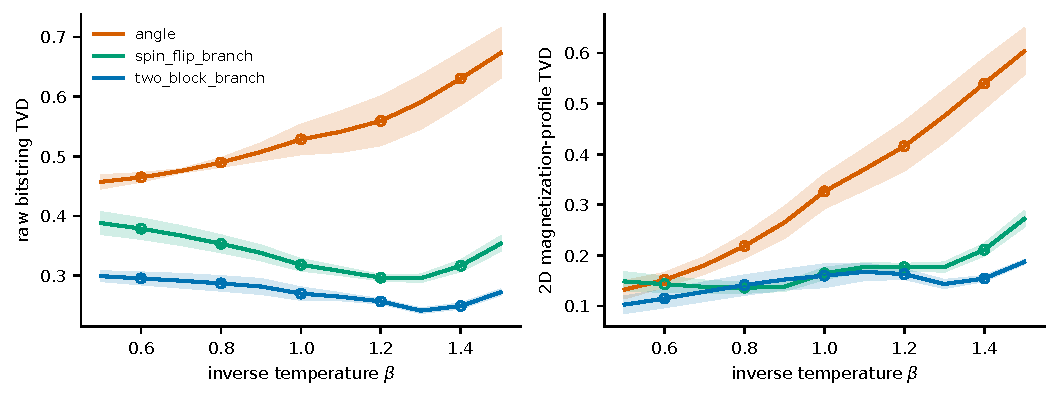
\includegraphics[width=\textwidth]{symmetry_figures/two_block_screen.pdf}
\caption{Exploratory two-block $Z_2^2$ screen. Held-out raw and two-block
magnetization-profile TVD for product, single-$Z_2$, and two-block-$Z_2^2$
inputs. Bands are one standard error across ten matched seeds; hollow markers
denote held-out temperatures.}
\label{fig:two-block}
\end{figure}

\paragraph{Asymmetric exchangeable targets.} A radial-shell state with a
frozen quartic shell law accepts two coordinates $(c_1,c_2)$ and preserves
permutation symmetry without enforcing spin flip. It improves the
weight-profile and permutation-averaged raw TVD in the reported screen, while
its unprocessed raw TVD is worse. The product and two-branch baselines receive
only $c_1$, whereas the radial model receives both $c_1$ and $c_2$; the result
therefore does not isolate symmetry matching from access to an additional
condition coordinate.

\begin{figure}[H]
\centering
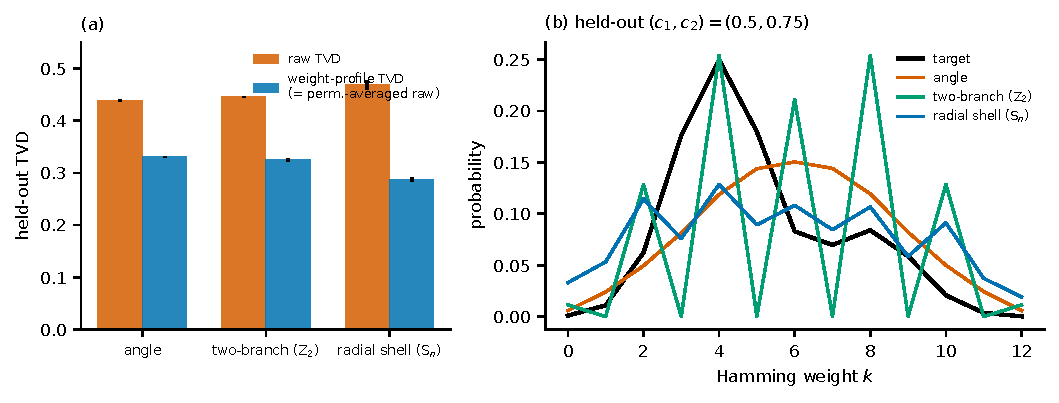
\includegraphics[width=\textwidth]{symmetry_figures/radial_shell.pdf}
\caption{Exploratory asymmetric radial-shell screen. Held-out raw and
weight-profile TVD and representative weight profiles are shown for the three
input families. The unequal condition information makes this a feasibility
screen rather than a controlled encoder comparison.}
\label{fig:radial}
\end{figure}

\section{Archived encoding comparison}
\label{app:encoding}

We tested two extensions of the single-angle product encoding on the
$n=19,s=0.50$ Gaussian task: noncommuting single-qubit reuploading and
two-qubit block-product inputs. None improved the tuned production encoder.
The study is supplementary because it followed a different development
protocol and its alternatives were not used in either production campaign.

\begin{table}[H]
\centering
\caption{Archived matched encoding comparison on the $n=19,s=0.50$
Gaussian task. Lower is better. The paired profile effect is relative to the
single-angle baseline; positive values are worse.}
\label{tab:encoding_benchmark}
\resizebox{\textwidth}{!}{%
\begin{tabular}{lcccc}
\toprule
encoding & structure & held-out profile TVD & held-out raw TVD & paired profile effect\\
\midrule
single angle & $L=1$ & $0.062\pm0.004$ & $0.348\pm0.006$ & baseline\\
noncommuting & $L=2$ & $0.072\pm0.009$ & $0.374\pm0.027$ & $+0.011$ [$+0.004,+0.017$]\\
block $ZZ$ & $\kappa=\pi/8$ & $0.070\pm0.008$ & $0.371\pm0.020$ & $+0.009$ [$+0.003,+0.015$]\\
block $ZZ$ & $\kappa=\pi/4$ & $0.071\pm0.014$ & $0.398\pm0.009$ & $+0.009$ [$-0.001,+0.017$]\\
\bottomrule
\end{tabular}}
\end{table}

\begin{figure}[H]
\centering
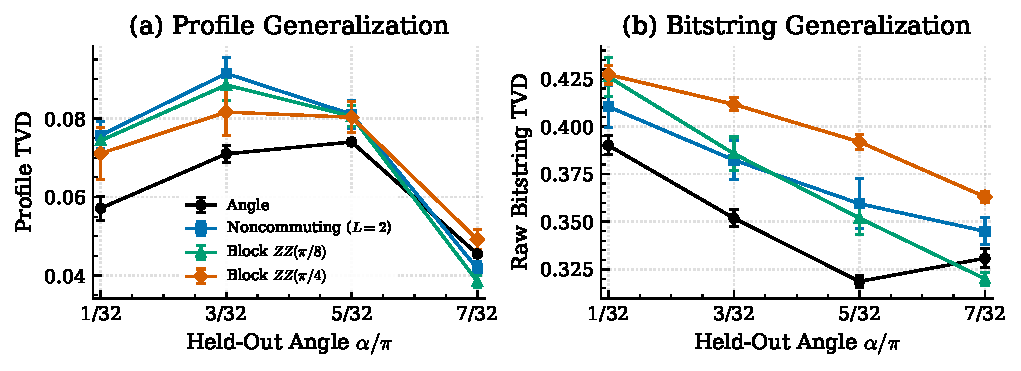
\includegraphics[width=\textwidth]{figures/encoding_benchmark.pdf}
\caption{Archived input-encoding comparison. The left panel reports held-out
conditional MMD and the right panel reports raw profile TVD for the four tested
architectures. Lower is better.}
\label{fig:encoding-benchmark}
\end{figure}

\section{Finite estimator audit}
\label{app:estimator-audit}

The separate estimator audit contains 21 deterministic synthetic cases over
qubit count, generator count, condition count, and condition dimension. It
uses bounded-degree and complete two-local generator families at $n=4$ and
$n=8$. Exact references are used where feasible; larger cases compare repeated
estimator draws. The audit records expectation and gradient-estimator errors,
runtime, memory, seeds, and content digests.

This is finite consistency and resource evidence only. It does not support an
asymptotic scaling claim, a statement about raw gradient magnitude, convergence
of the optimizer, or absence of barren plateaus. No full training run is
charged to this audit.

\section{Negative and boundary studies}

An eight-qubit pilot attempted joint conditioning on Gaussian location and
width. Its frozen design required adequate single-condition representability
before interpreting shared-model performance. Two narrow-width cells failed
that screen, so the study stopped. It supplies no evidence for
two-coordinate conditional generation and is retained as a negative result.

Older topology and ancilla studies remain archived under their original
protocols. They are not pooled with either production campaign. The two
symmetry screens above are supplementary exploratory evidence. Permutation
twirling is included only as target-symmetry-aware post-processing; it is not
a symmetry learned by the circuit.

\section{Campaign integrity and reproduction}
\label{app:reproduction}

The Gaussian and Curie--Weiss stores bind every run identity to a manifest,
role-tagged dataset, estimator streams, source digest, environment, code
revision, checkpoint, exact probability archive, invocation, runtime, and peak
memory. Stores reject undeclared identities, duplicate completion, and silent
reuse of partial results. Report, claim, table, and figure generators require
complete campaign state.

The Gaussian dependency closure includes a content-addressed snapshot of the
historical execution source. In particular, the archived
\texttt{encoding.py} has SHA-256
\texttt{0ec0d9d2903fd44684841721c9ffac9543f2c7f883e28f8ada09bb318e258338}.
The current live encoder is not substituted for that historical source.

The principal local reproduction commands are:
\begin{verbatim}
uv sync --frozen
uv run pytest -q
uv run ruff check src scripts tests
uv run python scripts/audit_gaussian_release.py
uv run python scripts/audit_curie_weiss_ancilla_release.py
uv run python scripts/run_curie_weiss_capacity_control.py run
uv run python scripts/run_curie_weiss_capacity_control.py summarize
(cd paper && latexmk -pdf main.tex)
\end{verbatim}

Exhaustive per-seed and per-condition tables remain in JSON, NPZ, and generated
TeX artifacts in the local review package. Keeping them machine-readable
preserves the audit trail without turning the supplement into a second report.


\end{document}
